% Options for packages loaded elsewhere
\PassOptionsToPackage{unicode}{hyperref}
\PassOptionsToPackage{hyphens}{url}
\documentclass[
  english,
  jou]{apa6}
\usepackage{xcolor}
\usepackage{amsmath,amssymb}
\setcounter{secnumdepth}{-\maxdimen} % remove section numbering
\usepackage{iftex}
\ifPDFTeX
  \usepackage[T1]{fontenc}
  \usepackage[utf8]{inputenc}
  \usepackage{textcomp} % provide euro and other symbols
\else % if luatex or xetex
  \usepackage{unicode-math} % this also loads fontspec
  \defaultfontfeatures{Scale=MatchLowercase}
  \defaultfontfeatures[\rmfamily]{Ligatures=TeX,Scale=1}
\fi
\usepackage{lmodern}
\ifPDFTeX\else
  % xetex/luatex font selection
\fi
% Use upquote if available, for straight quotes in verbatim environments
\IfFileExists{upquote.sty}{\usepackage{upquote}}{}
\IfFileExists{microtype.sty}{% use microtype if available
  \usepackage[]{microtype}
  \UseMicrotypeSet[protrusion]{basicmath} % disable protrusion for tt fonts
}{}
\makeatletter
\@ifundefined{KOMAClassName}{% if non-KOMA class
  \IfFileExists{parskip.sty}{%
    \usepackage{parskip}
  }{% else
    \setlength{\parindent}{0pt}
    \setlength{\parskip}{6pt plus 2pt minus 1pt}}
}{% if KOMA class
  \KOMAoptions{parskip=half}}
\makeatother
% Make \paragraph and \subparagraph free-standing
\makeatletter
\ifx\paragraph\undefined\else
  \let\oldparagraph\paragraph
  \renewcommand{\paragraph}{
    \@ifstar
      \xxxParagraphStar
      \xxxParagraphNoStar
  }
  \newcommand{\xxxParagraphStar}[1]{\oldparagraph*{#1}\mbox{}}
  \newcommand{\xxxParagraphNoStar}[1]{\oldparagraph{#1}\mbox{}}
\fi
\ifx\subparagraph\undefined\else
  \let\oldsubparagraph\subparagraph
  \renewcommand{\subparagraph}{
    \@ifstar
      \xxxSubParagraphStar
      \xxxSubParagraphNoStar
  }
  \newcommand{\xxxSubParagraphStar}[1]{\oldsubparagraph*{#1}\mbox{}}
  \newcommand{\xxxSubParagraphNoStar}[1]{\oldsubparagraph{#1}\mbox{}}
\fi
\makeatother
\usepackage{graphicx}
\makeatletter
\newsavebox\pandoc@box
\newcommand*\pandocbounded[1]{% scales image to fit in text height/width
  \sbox\pandoc@box{#1}%
  \Gscale@div\@tempa{\textheight}{\dimexpr\ht\pandoc@box+\dp\pandoc@box\relax}%
  \Gscale@div\@tempb{\linewidth}{\wd\pandoc@box}%
  \ifdim\@tempb\p@<\@tempa\p@\let\@tempa\@tempb\fi% select the smaller of both
  \ifdim\@tempa\p@<\p@\scalebox{\@tempa}{\usebox\pandoc@box}%
  \else\usebox{\pandoc@box}%
  \fi%
}
% Set default figure placement to htbp
\def\fps@figure{htbp}
\makeatother
% definitions for citeproc citations
\NewDocumentCommand\citeproctext{}{}
\NewDocumentCommand\citeproc{mm}{%
  \begingroup\def\citeproctext{#2}\cite{#1}\endgroup}
\makeatletter
 % allow citations to break across lines
 \let\@cite@ofmt\@firstofone
 % avoid brackets around text for \cite:
 \def\@biblabel#1{}
 \def\@cite#1#2{{#1\if@tempswa , #2\fi}}
\makeatother
\newlength{\cslhangindent}
\setlength{\cslhangindent}{1.5em}
\newlength{\csllabelwidth}
\setlength{\csllabelwidth}{3em}
\newenvironment{CSLReferences}[2] % #1 hanging-indent, #2 entry-spacing
 {\begin{list}{}{%
  \setlength{\itemindent}{0pt}
  \setlength{\leftmargin}{0pt}
  \setlength{\parsep}{0pt}
  % turn on hanging indent if param 1 is 1
  \ifodd #1
   \setlength{\leftmargin}{\cslhangindent}
   \setlength{\itemindent}{-1\cslhangindent}
  \fi
  % set entry spacing
  \setlength{\itemsep}{#2\baselineskip}}}
 {\end{list}}
\usepackage{calc}
\newcommand{\CSLBlock}[1]{\hfill\break\parbox[t]{\linewidth}{\strut\ignorespaces#1\strut}}
\newcommand{\CSLLeftMargin}[1]{\parbox[t]{\csllabelwidth}{\strut#1\strut}}
\newcommand{\CSLRightInline}[1]{\parbox[t]{\linewidth - \csllabelwidth}{\strut#1\strut}}
\newcommand{\CSLIndent}[1]{\hspace{\cslhangindent}#1}
\ifLuaTeX
\usepackage[bidi=basic,shorthands=off,]{babel}
\else
\usepackage[bidi=default,shorthands=off,]{babel}
\fi
\ifLuaTeX
  \usepackage{selnolig} % disable illegal ligatures
\fi
\setlength{\emergencystretch}{3em} % prevent overfull lines
\providecommand{\tightlist}{%
  \setlength{\itemsep}{0pt}\setlength{\parskip}{0pt}}
% Manuscript styling
\usepackage{upgreek}
\captionsetup{font=singlespacing,justification=justified}

% Table formatting
\usepackage{longtable}
\usepackage{lscape}
% \usepackage[counterclockwise]{rotating}   % Landscape page setup for large tables
\usepackage{multirow}		% Table styling
\usepackage{tabularx}		% Control Column width
\usepackage[flushleft]{threeparttable}	% Allows for three part tables with a specified notes section
\usepackage{threeparttablex}            % Lets threeparttable work with longtable

% Create new environments so endfloat can handle them
% \newenvironment{ltable}
%   {\begin{landscape}\centering\begin{threeparttable}}
%   {\end{threeparttable}\end{landscape}}
\newenvironment{lltable}{\begin{landscape}\centering\begin{ThreePartTable}}{\end{ThreePartTable}\end{landscape}}

% Enables adjusting longtable caption width to table width
% Solution found at http://golatex.de/longtable-mit-caption-so-breit-wie-die-tabelle-t15767.html
\makeatletter
\newcommand\LastLTentrywidth{1em}
\newlength\longtablewidth
\setlength{\longtablewidth}{1in}
\newcommand{\getlongtablewidth}{\begingroup \ifcsname LT@\roman{LT@tables}\endcsname \global\longtablewidth=0pt \renewcommand{\LT@entry}[2]{\global\advance\longtablewidth by ##2\relax\gdef\LastLTentrywidth{##2}}\@nameuse{LT@\roman{LT@tables}} \fi \endgroup}

% \setlength{\parindent}{0.5in}
% \setlength{\parskip}{0pt plus 0pt minus 0pt}

% Overwrite redefinition of paragraph and subparagraph by the default LaTeX template
% See https://github.com/crsh/papaja/issues/292
\makeatletter
\renewcommand{\paragraph}{\@startsection{paragraph}{4}{\parindent}%
  {0\baselineskip \@plus 0.2ex \@minus 0.2ex}%
  {-1em}%
  {\normalfont\normalsize\bfseries\itshape\typesectitle}}

\renewcommand{\subparagraph}[1]{\@startsection{subparagraph}{5}{1em}%
  {0\baselineskip \@plus 0.2ex \@minus 0.2ex}%
  {-\z@\relax}%
  {\normalfont\normalsize\itshape\hspace{\parindent}{#1}\textit{\addperi}}{\relax}}
\makeatother

\makeatletter
\usepackage{etoolbox}
\patchcmd{\maketitle}
  {\section{\normalfont\normalsize\abstractname}}
  {\section*{\normalfont\normalsize\abstractname}}
  {}{\typeout{Failed to patch abstract.}}
\patchcmd{\maketitle}
  {\section{\protect\normalfont{\@title}}}
  {\section*{\protect\normalfont{\@title}}}
  {}{\typeout{Failed to patch title.}}
\makeatother

\usepackage{xpatch}
\makeatletter
\xapptocmd\appendix
  {\xapptocmd\section
    {\addcontentsline{toc}{section}{\appendixname\ifoneappendix\else~\theappendix\fi: #1}}
    {}{\InnerPatchFailed}%
  }
{}{\PatchFailed}
\makeatother
\keywords{Industrial emissions, Acid rain, Sulfur dioxide (SO2), Nitrogen oxides (NOx), Clean Air Act Amendments, Acid Rain Program, Redlining (HOLC), Racial wealth gap, Social Vulnerability Index (SVI), Transboundary pollution, Atmospheric deposition, Biogeochemical cycling, Hubbard Brook Experimental Forest, Spatial analysis}
\usepackage{dblfloatfix}


\usepackage{csquotes}
\usepackage[version=4]{mhchem}
\usepackage{float}
\usepackage{bookmark}
\IfFileExists{xurl.sty}{\usepackage{xurl}}{} % add URL line breaks if available
\urlstyle{same}
\hypersetup{
  pdftitle={Inequality-Driven Socio-Economic Origins of Industrial Emissions and The Resultant Transboundary Corollaries of Acid Rain in Forest Ecosystems},
  pdfauthor={Suzanne Pierre1, Pa-Shun D. Hawkins1,2, \& Robert J. Dellinger1,3},
  pdflang={en-EN},
  pdfkeywords={Industrial emissions, Acid rain, Sulfur dioxide (SO2), Nitrogen oxides (NOx), Clean Air Act Amendments, Acid Rain Program, Redlining (HOLC), Racial wealth gap, Social Vulnerability Index (SVI), Transboundary pollution, Atmospheric deposition, Biogeochemical cycling, Hubbard Brook Experimental Forest, Spatial analysis},
  hidelinks,
  pdfcreator={LaTeX via pandoc}}

\title{\textbf{Inequality-Driven Socio-Economic Origins of Industrial Emissions and The Resultant Transboundary Corollaries of Acid Rain in Forest Ecosystems}}
\author{Suzanne Pierre\textsuperscript{1}, Pa-Shun D. Hawkins\textsuperscript{1,2}, \& Robert J. Dellinger\textsuperscript{1,3}}
\date{}


\shorttitle{Emissions/Inequality Research Project}

\authornote{

We gratefully acknowledge the Hubbard Brook Long Term Ecological Research (LTER) program for access to long-term ecological observations and data products. We also thank the U.S. Environmental Protection Agency for public access to emissions datasets, including the National Emissions Inventory (NEI) and the Clean Air Markets Division Acid Rain Program (ARP). Digitized HOLC ``Residential Security'' maps were obtained from the Mapping Inequality: Redlining in New Deal America project (Digital Scholarship Lab), and measures of social vulnerability were derived from the CDC/ATSDR Social Vulnerability Index (SVI).

The authors made the following contributions. Suzanne Pierre: Project administration, Conceptualization, Writing - Original Draft Preparation, Writing - Review \& Editing, Supervision; Pa-Shun D. Hawkins: Conceptualization, Writing - Original Draft Preparation, Writing - Review \& Editing, Data curation, Methodology, Formal analysis, Visualization; Robert J. Dellinger: Conceptualization, Writing - Original Draft Preparation, Writing - Review \& Editing, Data curation, Methodology, Formal analysis, Visualization.

Correspondence concerning this article should be addressed to Suzanne Pierre, 887 Sonoma Ave Unit 23 Santa Rosa, CA 95404. E-mail: \href{mailto:spierre.cel@gmail.com}{\nolinkurl{spierre.cel@gmail.com}}

}

\affiliation{\vspace{0.5cm}\textsuperscript{1} Critical Ecology Lab, Independent Research \& 501(c)3 Nonprofit Organization\\\textsuperscript{2} Institute of the Environment and Sustainability, University of California, Los Angeles\\\textsuperscript{3} Department of Atmospheric and Oceanic Sciences, University of California, Los Angeles}

\abstract{%
This study explores the intersection of socio-economic inequality and industrial emissions, with a focus on socio-economic and racial stratification as a key driver of environmental degradation, particularly acid rain, in forest ecosystems. We hypothesize that regions with higher socio-economic inequality, especially those with a significant racial wealth gap, are disproportionately impacted by industrial emissions, which contribute to acid rain. Our analysis integrates emissions data from the EPA National Emissions Inventory and Acid Rain Program, wealth inequality data from Census records, and long-term ecological data from the NSF LTER network.
}



\begin{document}
\maketitle

\section{Introduction}\label{introduction}

Air pollution is not placed randomly; its sources follow geographies of exclusion, marked by notions of race and class, and sedimented through decades of policy decisions (\citeproc{ref-hailemariamcarbonemissions}{Hailemariam, Dzhumashev, \& Shahbaz, 2020}; \citeproc{ref-schellsystemicracism}{Schell et al., 2020}). One of the most enduring cartographies of these injustices is inscribed within the U.S . Federal Government's Home Owners' Loan Corporation (HOLC) ``Residential Security'' maps from the 1930s, which institutionalized racial segregation through ranking mortgage risk ratings and providing specific locations for investments of industrial activity (\citeproc{ref-nelsonmappinginequality}{Nelson, Winling, Marciano, Connolly, \& Ayers, 2020}). Nearly a century later, these maps continue to predict where environmental hazards and harms concentrate and where they don't (\citeproc{ref-desrochessocioeco}{Des Roches et al., 2021}; \citeproc{ref-estienhistoricalredlining}{Estien, Omar, Fidino, Wilkinson, \& Morello-Frosch, 2023}; \citeproc{ref-tessumracialdisparitiespm25}{Tessum, Hill, Apte, Chambliss, \& Marshall, 2021}).

One of the most well-known atmospheric hazards of the late 20th century is acid rain, primarily driven by sulfur dioxide (\ce{SO2}) and nitrogen oxide (\ce{NOx}) emissions from fossil-fuel-powered electric utilities and coal burning activities (\citeproc{ref-driscollacidrain}{Driscoll et al., 2001}). Hubbard Brook Experimental Forest in New Hampshire became the primary site for documenting the biogeochemical consequences of these emissions for decades. Long-term monitoring at Hubbard Brook provided the first empirical evidence that acidic deposition from upwind sources was altering soil chemistry and restructuring forest ecosystems. It was here that the link between distant emissions and local ecological degradation was scientifically grounded and studied through isotope geochemistry, catalyzing the 1990 Clean Air Act Amendments (CAAA) and the establishment of the Acid Rain Program (ARP) -the first cap and trade system for atmospheric pollutants (\citeproc{ref-driscollacidrain}{Driscoll et al., 2001}; \citeproc{ref-likensdiscoveryacidrain}{Likens \& Bailey, 2014}; \citeproc{ref-likenscenturychange}{Likens, Buso, Bernhardt, \& Rosi, 2021}; \citeproc{ref-mitchellstableisotopes}{Mitchell et al., 2001}) But while the research at Hubbard Brook clarified the where and what of acid rain, it left open the who and why? Who lives downwind of these emissions, and why are those locations chosen?

This study interrogates the intersection of historical segregation, contemporary inequality, and the geography of atmospheric pollution to ask: \textbf{Does structural inequality shape the sources and quantity of emissions that contribute to acid rain?} Our hypotheses are two-fold. First, we hypothesize that areas of higher social vulnerability (e.g, lower median household income), will exhibit higher emissions per census tract. Second, we hypothesize that power plant pollution continues to fall disproportionately on neighborhoods historically graded ``hazardous'' (D) or ``declining'' (C) by HOLC due to structural conditions that rendered these areas as politically marginal and economically expendable. To test this, we integrate long-term \ce{SO2} and \ce{NOx} emissions data from the EPA National Emissions Inventory (NEI) and the EPA ARP with digitized HOLC maps and the CDC's Social Vulnerability Index. This spatial synthesis allows us to trace not only the environmental consequences of polluting industries but also the racial and economic geographies that shape their placement and persistence. Our analytical anchor remains the northeastern U.S., particularly the states implicated in emissions transport to Hubbard Brook, where isotopic signatures of acid deposition have been traced to seven states of interest. By situating Hubbard Brook within a broader socio-political context, we intend to reframe acid rain as not merely an ecological consequence, but as a spatialized expression of inequality-based emissions. In telling this story, we aim to expand the narrative of atmospheric science: from one focused solely on emissions and deposition to one that reckons with the social drivers of environmental change.

\begin{figure}[H]

{\centering 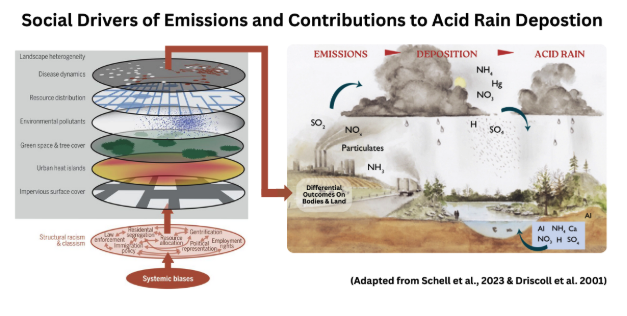
\includegraphics[width=1\linewidth]{Figures/CEL_Visual_Abstract} 

}

\caption[Social drivers of emissions and acid-rain deposition.]{Social drivers of emissions and contributions to acid-rain deposition. The left panel (stacked layers) depicts how structural racism and classed systems shape urban biophysical conditions (e.g., landscape heterogeneity, disease dynamics, resource distribution, pollutants, green space/tree cover, urban heat, impervious surfaces), which in turn influence emission sources. The right panel illustrates emissions, atmospheric transport and deposition, and formation of acid rain, with downstream effects on soils and waters.}\label{fig:visual-abstract}
\end{figure}

\protect\phantomsection\label{refs}
\begin{CSLReferences}{1}{0}
\bibitem[\citeproctext]{ref-desrochessocioeco}
Des Roches, S., Brans, K. I., Lambert, M. R., Rivkin, L. R., Savage, A. M., Schell, C. J., \& Alberti, M. (2021). Socio-eco-evolutionary dynamics in cities. \emph{Evolutionary Applications}, \emph{14}(1), 248--267. \url{https://doi.org/10.1111/eva.13065}

\bibitem[\citeproctext]{ref-driscollacidrain}
Driscoll, C. T., Lawrence, G. B., Bulger, A. J., Butler, T. J., Cronan, C. S., Eagar, C., \& Weathers. (2001). Acid rain revisited: Advances in scientific understanding since the passage of the 1970 and 1990 clean air act amendments. \emph{Hubbard Brook Research Foundation. Science Links' Publication}, \emph{1}.

\bibitem[\citeproctext]{ref-estienhistoricalredlining}
Estien, C., Omar, M., Fidino, C. E., Wilkinson, R., \& Morello-Frosch, C. J. (2023). \emph{Historical redlining impacts wildlife biodiversity across california}.

\bibitem[\citeproctext]{ref-hailemariamcarbonemissions}
Hailemariam, A., Dzhumashev, R., \& Shahbaz, M. (2020). Carbon emissions, income inequality and economic development. \emph{Empirical Economics}, \emph{59}(3), 1139--1159. \url{https://doi.org/10.1007/s00181-019-01664-x}

\bibitem[\citeproctext]{ref-likensdiscoveryacidrain}
Likens, G. E., \& Bailey, S. W. (2014). The discovery of acid rain at the hubbard brook experimental forest: A story of collaboration and long-term research. In D. C. Hayes, S. L. Stout, R. H. Crawford, \& A. P. Hoover (Eds.), \emph{USDA forest service experimental forests and ranges} (pp. 463--482). Springer New York. \url{https://doi.org/10.1007/978-1-4614-1818-4_20}

\bibitem[\citeproctext]{ref-likenscenturychange}
Likens, G. E., Buso, D. C., Bernhardt, E. S., \& Rosi, E. (2021). A century of change: Reconstructing the biogeochemical history of hubbard brook. \emph{Hydrological Processes}, \emph{35}(6). \url{https://doi.org/10.1002/hyp.14256}

\bibitem[\citeproctext]{ref-mitchellstableisotopes}
Mitchell, M. J., Mayer, B., Bailey, S. W., Hornbeck, J. W., Alewell, C., Driscoll, C. T., \& Likens, G. E. (2001). Use of stable isotope ratios for evaluating sulfur sources and losses at the hubbard brook experimental forest. \emph{Water, Air, and Soil Pollution}, \emph{130}(1/4), 75--86. \url{https://doi.org/10.1023/a:1012295301541}

\bibitem[\citeproctext]{ref-nelsonmappinginequality}
Nelson, R. K., Winling, L., Marciano, R., Connolly, N., \& Ayers, E. L. (2020). \emph{Mapping inequality: Redlining in new deal america}. Digital Scholarship Lab.

\bibitem[\citeproctext]{ref-schellsystemicracism}
Schell, C. J., Dyson, K., Fuentes, T. L., Des Roches, S., Harris, N. C., Miller, D. S., \& Lambert, M. R. (2020). The ecological and evolutionary consequences of systemic racism in urban environments. \emph{Science (New York, N.Y.)}, \emph{369}(6510). \url{https://doi.org/10.1126/science.aay4497}

\bibitem[\citeproctext]{ref-tessumracialdisparitiespm25}
Tessum, C. W., Hill, J. D., Apte, J. S., Chambliss, S. E., \& Marshall, J. D. (2021). Racial disparities in air pollution exposure in the united states. \emph{Science Advances}, \emph{7}(2). \url{https://doi.org/10.1126/sciadv.abe0646}

\end{CSLReferences}


\end{document}
